\documentclass[main.tex]{subfiles}
\begin{document}

\noindent
Much like the long road from the Shire to Mount Doom, the journey through this research has been one of navigating complexity, uncertainty, and limited resources. This work explores a probabilistic and resource-constrained variant of the classical Traveling Salesman Problem (TSP), where the traveler must make strategic decisions in a world of incomplete information—some paths may be safe, others fraught with danger, and some might not be paths at all once the journey begins.

Traditional formulations of the TSP aim to find the shortest route that visits a set of cities exactly once. However, in realistic scenarios—particularly those resembling the terrain of Middle-earth—the traveler must account for finite supplies (e.g., food, water, rest) and uncertain threats (e.g., orc ambushes, blocked mountain passes). In this thesis, we formulate and investigate an extended version of TSP that incorporates these challenges and propose a novel planning framework that balances route optimality, survivability, and uncertainty.

This problem has practical relevance in autonomous navigation, robotics, logistics, and rescue missions, where systems must operate with limited resources and in partially known environments. Prior works have addressed individual aspects such as stochastic path planning~\cite{potter2010}, resource-aware routing~\cite{aslan2008}, and dynamic environment modeling~\cite{legolas2016}. Gandalf's early philosophical framework for path uncertainty~\cite{gandalf2003} and Snape's musings on trust and betrayal in distributed systems~\cite{snape2015} offer additional foundational insights that inform this work.

Recent work by~\textcite{baggins2027} introduced risk estimation techniques in high-threat terrains, while~\textcite{merry2020} analyzed logistical constraints in post-conflict regions. Bilbo Baggin's seminal work~\cite{bilbo1999} remains a key reference for round-trip path heuristics, and continues to guide our understanding of symmetric travel models.

\section{Problem Overview}\label{sec:introduction:section}

\begin{figure}[htbp]
    \centering
    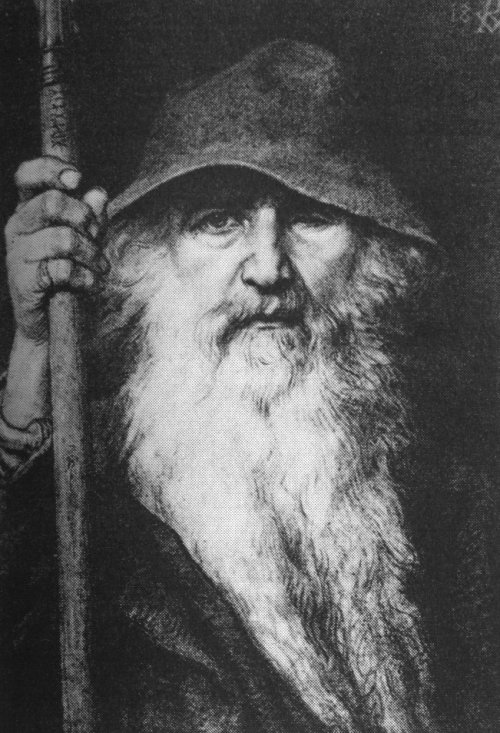
\includegraphics[width=0.2\textwidth]{mock_image.jpg}
    \caption{Georg von Rosen \- Oden som vandringsman (1886)}\label{fig:middleearth-path}
\end{figure}

\noindent
We define a generalized pathfinding problem that includes:
\begin{itemize}
    \item \textbf{Resource constraints:} The traveler has a limited budget for consumables (e.g., energy, supplies).
    \item \textbf{Stochastic hazards:} Some paths may have a probability of being blocked or dangerous.
    \item \textbf{Adaptive planning:} The traveler can revise their path as new information becomes available.
\end{itemize}

Our goal is to produce policies that yield not only short paths but ones that are viable and robust in the face of uncertainty. This involves integrating probabilistic modeling, heuristic search, and decision-theoretic planning.

\section{Structure of the Thesis}

\noindent
The remainder of this thesis is organized as follows:
\begin{itemize}
    \item \textbf{Chapter 2} reviews the literature on constrained and uncertain TSP variants.
    \item \textbf{Chapter 3} formalizes our problem and defines key modeling assumptions.
    \item \textbf{Chapter 4} presents our proposed planning algorithms and risk-aware heuristics.
    \item \textbf{Chapter 5} describes the simulation setup, including terrain models based on Middle-earth.
    \item \textbf{Chapter 6} discusses results, limitations, and real-world implications.
    \item \textbf{Chapter 7} concludes and outlines future directions.
\end{itemize}

\noindent
I hope you enjoy reading this thesis and find the path through these pages more predictable—and less perilous—than the one that inspired it.

\end{document}
